\documentclass[a4paper,11pt,dvipdfmx]{jsarticle}


% 数式
\usepackage{amsmath,amsfonts}
\usepackage{bm}

% 画像
\usepackage[dvipdfmx]{graphicx}

% 図形
\usepackage{tikz}
\usetikzlibrary{shapes.geometric}
\usetikzlibrary {shapes.misc}
\usetikzlibrary{shapes, arrows.meta, positioning}

% ソースコード
\usepackage{listings,jlisting,color}
\lstset{
basicstyle={\ttfamily},
identifierstyle={\small},
commentstyle={\smallitshape},
keywordstyle={\small\bfseries},
ndkeywordstyle={\small},
stringstyle={\small\ttfamily},
frame={tb},
breaklines=true,
columns=[l]{fullflexible},
numbers=left,
xrightmargin=0zw,
xleftmargin=3zw,
numberstyle={\scriptsize},
stepnumber=1,
numbersep=1zw,
lineskip=-0.5ex
}
\renewcommand{\lstlistingname}{ソースコード}

\newcommand*{\inteltable}[5]{
    \begin{tabular}{l|c}
        #1 & #2 \\ \hline 
        \multicolumn{2}{c}{#3} \\ 
        \multicolumn{2}{c}{#4} \\ 
        \multicolumn{2}{c}{#5} 
    \end{tabular}
}

\begin{document}

\title{インテリジェントシステム レポート課題1}
\author{21T2166D 渡辺大樹}
\date{\today}
\maketitle
\section{A*探索アルゴリズムでの探索}
\subsection{(a)AradからBucharestまで}
\subsubsection{A1 $f_1(n)=g(n)+D(n)$を用いた探索}
$f_1(n)=g(n)+D(n)$の評価関数を用いて探索を行った結果、Bucharestのノード情報は[14, Bucharest, 418, 418, 10]となった。

見つかった経路はArad→Sibin→Rimnicu Vilces→Pitesti→Bucharestとなった。

ゴールが見つかった時点でのfrontierはF値の順に \\ \noindent
[3, Timisoara, 118, 447, 1], \\ \noindent
[4, Zerind, 75, 449, 1], \\ \noindent
[9, Craiova, 366, 526, 8], \\ \noindent
[11, Sibiu, 300, 553, 8], \\ \noindent
[13, Sibiu, 338, 591, 6], \\ \noindent
[16, Rimnicu Vilces, 414, 607, 10], \\ \noindent
[15, Craiova, 455, 615, 10], \\ \noindent
[5, Arad, 280, 646, 2], \\ \noindent
[7, Oradea, 291, 671, 2], \\ \noindent
となった。

以下に実際に展開されたSearch Treeを示す。


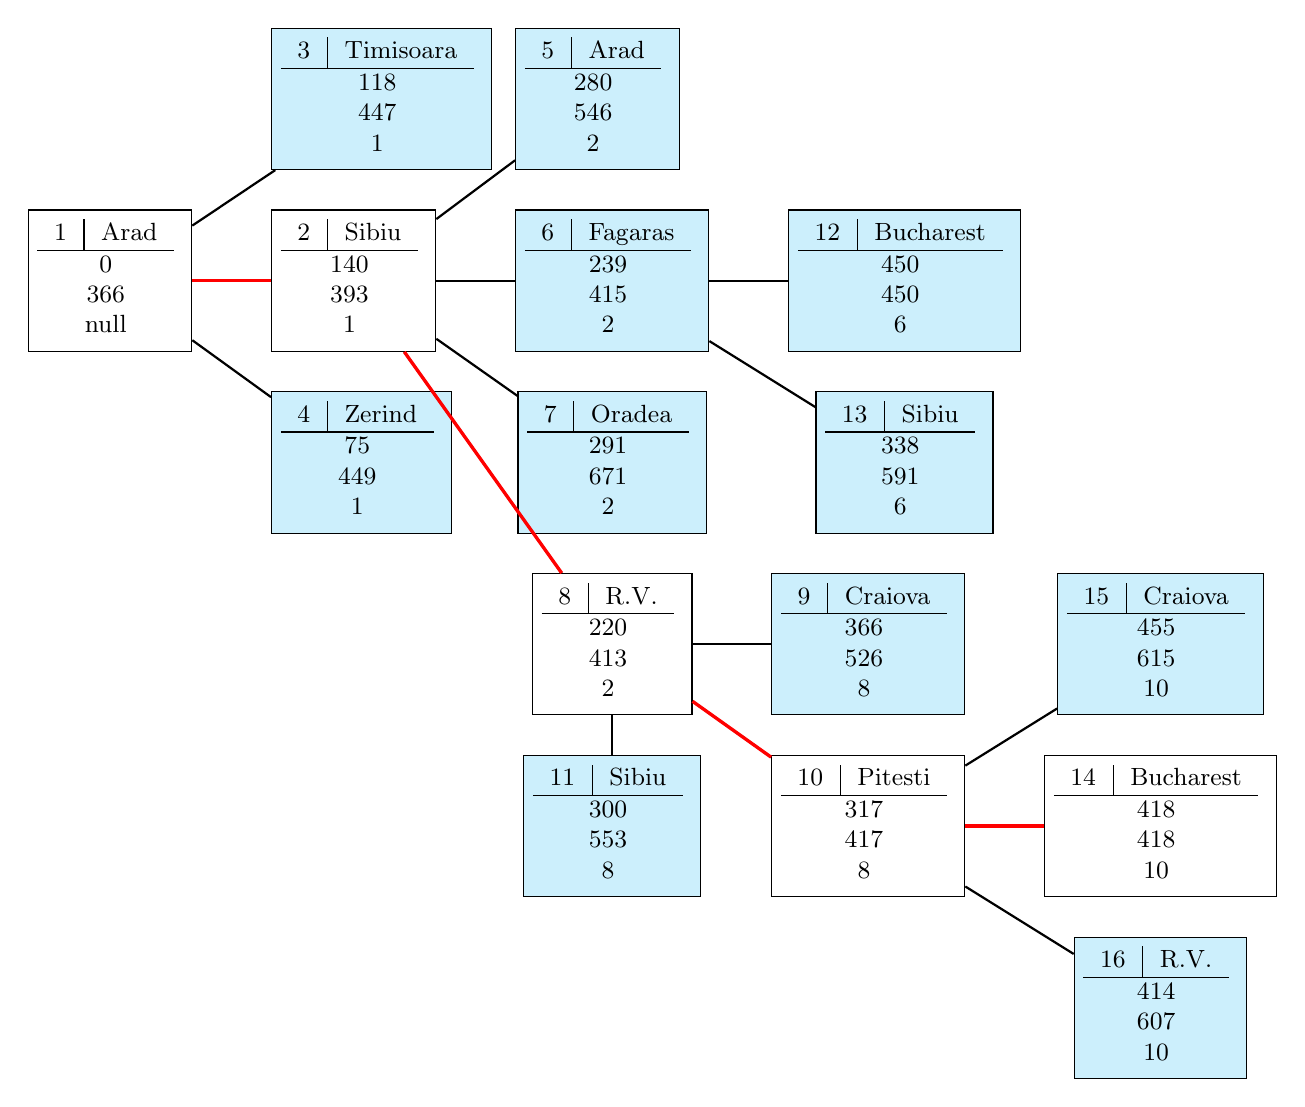
\begin{tikzpicture}[node distance=1cm, auto, >={Latex[width=1mm,length=1mm]}, align=center]

\tikzset{
    node/.style = {rectangle, draw, minimum width=1.5cm, minimum height=1ex, font=\small},
    leaf/.style = {rectangle, draw, fill=cyan!20, minimum width=1.5cm, minimum height=1ex, font=\small},
    root/.style = {rectangle, draw, fill=white, minimum width=1.5cm, minimum height=1ex, font=\small},
    edge from parent/.style = {draw, thick, black},
    edge from parent path={(\tikzparentnode.south) -- (\tikzchildnode.north)},
}

% Define nodes
\node[root] (A1) {\inteltable{1}{Arad}{0}{366}{null}};
\node[node, right=of A1] (B2) {\inteltable{2}{Sibiu}{140}{393}{1}};
\node[leaf, above right=0.5cm and 1cm of A1] (A3) {\inteltable{3}{Timisoara}{118}{447}{1}};
\node[leaf, below right=0.5cm and 1cm of A1] (A4) {\inteltable{4}{Zerind}{75}{449}{1}};

\node[leaf, above right=0.5cm and 1cm of B2] (B5) {\inteltable{5}{Arad}{280}{546}{2}};
\node[leaf, right=of B2] (B6) {\inteltable{6}{Fagaras}{239}{415}{2}};
\node[leaf, below=0.5cm of B6] (B7) {\inteltable{7}{Oradea}{291}{671}{2}};
\node[node, below=0.5cm of B7] (B8) {\inteltable{8}{R.V.}{220}{413}{2}};

\node[leaf, right=of B6] (B12) {\inteltable{12}{Bucharest}{450}{450}{6}};
\node[leaf, below=0.5cm of B12] (B13) {\inteltable{13}{Sibiu}{338}{591}{6}};

\node[leaf, right=of B8] (B9) {\inteltable{9}{Craiova}{366}{526}{8}};
\node[node, below=0.5cm of B9] (B10) {\inteltable{10}{Pitesti}{317}{417}{8}};

\node[node, right=of B10] (B14) {\inteltable{14}{Bucharest}{418}{418}{10}};
\node[leaf, above=0.5cm of B14] (B15) {\inteltable{15}{Craiova}{455}{615}{10}};
\node[leaf, below=0.5cm of B14] (B16) {\inteltable{16}{R.V.}{414}{607}{10}};

\node[leaf, below=0.5cm of B8] (B11) {\inteltable{11}{Sibiu}{300}{553}{8}};

% Draw edges
\draw[edge from parent] (A1) -- (B2);
\draw[edge from parent] (A1) -- (A3);
\draw[edge from parent] (A1) -- (A4);

\draw[edge from parent] (B2) -- (B5);
\draw[edge from parent] (B2) -- (B6);
\draw[edge from parent] (B2) -- (B7);
\draw[edge from parent] (B2) -- (B8);

\draw[edge from parent] (B6) -- (B12);
\draw[edge from parent] (B6) -- (B13);

\draw[edge from parent] (B8) -- (B9);
\draw[edge from parent] (B8) -- (B10);

\draw[edge from parent] (B10) -- (B14);
\draw[edge from parent] (B10) -- (B15);
\draw[edge from parent] (B10) -- (B16);
\draw[edge from parent] (B8) -- (B11);

% Draw red edges
\draw[red, very thick] (A1) -- (B2);
\draw[red, very thick] (B2) -- (B8);
\draw[red, very thick] (B8) -- (B10);
\draw[red, very thick] (B10) -- (B14);

\end{tikzpicture}

\subsubsection{A2 $f_1(n)=g(n)+2 \cdot D(n)$を用いた探索}
$f_1(n)=g(n)+2 \cdot D(n)$の評価関数を用いて探索を行った結果、Bucharestのノード情報は[9, Bucharest, 450, 450, 6]となった。

見つかった経路はArad→Sibin→Fagaras→Bucharestとなった。

ゴールが見つかった時点でのfrontierはF値の順に \\ \noindent
[8, Rimnicu Vilces, 220, 606, 2], \\ \noindent
[3, Timisoara, 118, 776, 1], \\ \noindent
[4, Zerind, 75, 823, 1], \\ \noindent
[10, Sibiu, 338, 844, 6], \\ \noindent
[5, Arad, 280, 1012, 2], \\ \noindent
[7, Oradea, 291, 1051, 2] \\ \noindent
となった。

以下に実際に展開されたSearch Treeを示す。
\\

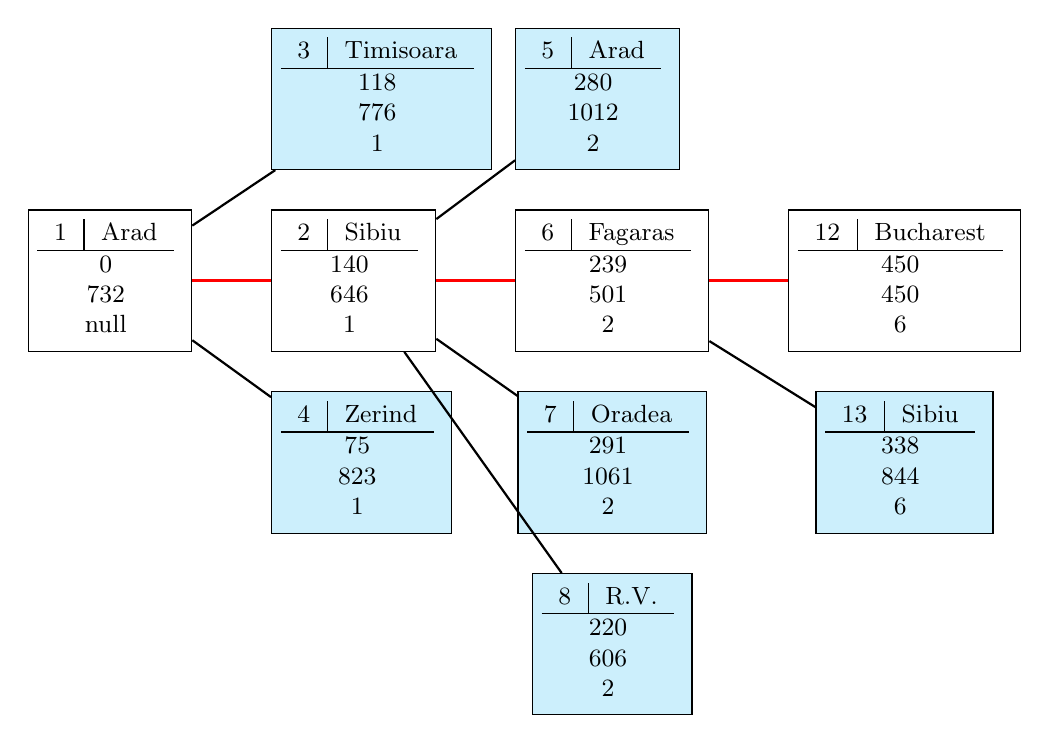
\begin{tikzpicture}[node distance=1cm, auto, >={Latex[width=1mm,length=1mm]}, align=center]

    \tikzset{
        node/.style = {rectangle, draw, minimum width=1.5cm, minimum height=1ex, font=\small},
        leaf/.style = {rectangle, draw, fill=cyan!20, minimum width=1.5cm, minimum height=1ex, font=\small},
        root/.style = {rectangle, draw, fill=white, minimum width=1.5cm, minimum height=1ex, font=\small},
        edge from parent/.style = {draw, thick, black},
        edge from parent path={(\tikzparentnode.south) -- (\tikzchildnode.north)},
    }
    
    % Define nodes
    \node[root] (A1) {\inteltable{1}{Arad}{0}{732}{null}};
    \node[node, right=of A1] (B2) {\inteltable{2}{Sibiu}{140}{646}{1}};
    \node[leaf, above right=0.5cm and 1cm of A1] (A3) {\inteltable{3}{Timisoara}{118}{776}{1}};
    \node[leaf, below right=0.5cm and 1cm of A1] (A4) {\inteltable{4}{Zerind}{75}{823}{1}};
    
    \node[leaf, above right=0.5cm and 1cm of B2] (B5) {\inteltable{5}{Arad}{280}{1012}{2}};
    \node[node, right=of B2] (B6) {\inteltable{6}{Fagaras}{239}{501}{2}};
    \node[leaf, below=0.5cm of B6] (B7) {\inteltable{7}{Oradea}{291}{1061}{2}};
    \node[leaf, below=0.5cm of B7] (B8) {\inteltable{8}{R.V.}{220}{606}{2}};
    
    \node[node, right=of B6] (B12) {\inteltable{12}{Bucharest}{450}{450}{6}};
    \node[leaf, below=0.5cm of B12] (B13) {\inteltable{13}{Sibiu}{338}{844}{6}};
    
    % Draw edges
    \draw[edge from parent] (A1) -- (B2);
    \draw[edge from parent] (A1) -- (A3);
    \draw[edge from parent] (A1) -- (A4);
    
    \draw[edge from parent] (B2) -- (B5);
    \draw[edge from parent] (B2) -- (B6);
    \draw[edge from parent] (B2) -- (B7);
    \draw[edge from parent] (B2) -- (B8);
    
    \draw[edge from parent] (B6) -- (B12);
    \draw[edge from parent] (B6) -- (B13);
    
    % Draw red edges
    \draw[red, very thick] (A1) -- (B2);
    \draw[red, very thick] (B2) -- (B6);
    \draw[red, very thick] (B6) -- (B12);
    
\end{tikzpicture}

\subsection{(b)LugojからBucharestまで}
\subsubsection{A1 $f_1(n)=g(n)+D(n)$を用いた探索}
$f_1(n)=g(n)+D(n)$の評価関数を用いて、LugojからBucharestまでの探索を行った結果、Bucharestのノード情報は[21, Bucharest, 504, 504, 11]となった。
見つかった経路はLugoj→Mehadin→Droveta→Craiova→Pitesti→Bucharestとなった。

ゴールが見つかった時点でのfrontierはF値の順に \\ \noindent
[16, Lugoj, 280, 524, 6], \\ \noindent
[15, Droveta, 285, 527, 5], \\ \noindent
[19, Mahadia, 292, 533, 14], \\ \noindent
[18, Lugoj, 290, 534, 9], \\ \noindent
[17, Droveta, 295, 537, 9], \\ \noindent
[10, Timisoara, 251, 580, 5], \\ \noindent
[13, Arad, 229, 595, 3], \\ \noindent
[12, Rimnicu Vilces, 411, 604, 8], \\ \noindent
[10, Droveta, 385, 627, 8], \\ \noindent
[20, Timisoara, 333, 662, 14], \\ \noindent
[23, Rimnicu Vilces, 500, 693, 11], \\ \noindent
[22, Craiova, 541, 701, 11], \\ \noindent

となった。


\subsubsection{A2 $f_1(n)=g(n)+2 \cdot D(n)$を用いた探索}
$f_1(n)=g(n)+2 \cdot D(n)$の評価関数を用いて、LugojからBucharestまでの探索を行った結果、Bucharestのノード情報は[13, Bucharest, 504, 504, 11]となった.
見つかった経路はLugoj→Mahadia→Droveta→Craiova→Pitesti→Bucharestとなった。

ゴールが見つかった時点でのfrontierはF値の順に \\ \noindent
[6, Mahadia, 210, 692, 5], \\ \noindent
[9, Mahadia, 220, 702, 4], \\ \noindent
[3, Timisoara, 111, 769, 1], \\ \noindent
[12, Rimnicu Vilces, 411, 797, 8], \\ \noindent
[14, Craiova, 541, 861, 11], \\ \noindent
[10, Droveta, 385, 869, 8], \\ \noindent
[15, Rimnicu Vilces, 500, 886, 11], \\ \noindent
[7, Timisoara, 251, 909, 5], \\ \noindent

となった。

\section{ヒューリスティック関数の許容性について}
この課題では以下の$h_a \sim h_f$が許容的であるかを調べる。

許容的とは、すべてのノードに対してヒューリスティック関数が示す予想最小コスト$h(n)$が
そのノードからの実際の最小コストとなる$h^*(n)$以下になることをいう。

すなわち以下に与えられる関数$h_a \sim h_f$に対し、すべてのnで$h_x(n) \leq h^*(n)$を言えればその関数は許容的であるといえる。

ただし、$1 \leq i \leq k$の$i$について$h_i(n) \leq h^*(n)$(すなわち許容的)である。
\subsection{$h_a(n)$}
$h_a(n)$は
\begin{equation*}
    h_a(n) = \sum_{i=1}^{k}h_i(n)
\end{equation*}
の関数となる。

この関数$h_a(n)$が$h^*(n)$以下になるとき、許容的であるといえる。
ここで$h_i(n) \leq h^*(n)$より$h_1(n), h_2(n) = h^*(n)$であるとすると少なくとも$h_a(n)$は
\begin{equation*}
    h_a(n) \geq 2 \cdot h^*(n)
\end{equation*}
であるといえる。

したがって$h_a(n)$は許容的ではない。

\subsection{$h_b(n),h_c(n)$}
$h_b(n)$は
\begin{equation*}
    h_b(n) = \max\{h_1(n),h_2(n),h_3(n),\cdots,h_k(n)\}
\end{equation*}
の関数となる。

この関数$h_b(n)$が$h^*(n)$以下になるとき、許容的であるといえる。
$\max$関数は$h_1(n),h_2(n),h_3(n),\cdots,h_k(n)$の関数の中から最大となる関数を選ぶ関数である。
$h_i(n) \leq h^*(n)$より任意の$h_i(n)$において許容的となるため、$\max$関数によってどの関数が選ばれても$h_b(n)$は許容的である。

$h_c(n)$も同様であり、$h_c(n)$は
\begin{equation*}
    h_c(n) = \min\{h_1(n),h_2(n),h_3(n),\cdots,h_k(n)\}
\end{equation*}
の関数となる。

上記にあるようにこちらも$\min$関数の働きを考えれば$h_c(n)$は許容的であるといえる。

\subsection{$h_d(n)$}
$h_d(n)$は
\begin{equation*}
    h_d(n) = \prod_{i=1}^{k}h_i(n)
\end{equation*}
の関数となる。

この関数$h_d(n)$が$h^*(n)$以下になるとき、許容的であるといえる。
ここで$h_i(n) \leq h^*(n)$より$h_1(n), h_2(n) = h^*(n)$であるとすると少なくとも$h_d(n)$は
\begin{equation*}
    h_d(n) \geq \{h^*(n)\}^2
\end{equation*}
であるといえる。

したがって$h_d(n)$は許容的ではない。

\subsection{$h_e(n)$}
$h_e(n)$は
\begin{equation*}
    h_e(n) = \frac{1}{k}\sum_{i=1}^{k}h_i(n)
\end{equation*}
の関数となる。

この関数$h_e(n)$が$h^*(n)$以下になるとき、許容的であるといえる。
ここで$h_i(n) \leq h^*(n)$より、$h_i(n)$をすべてが最大値である$h_1(n),h_2(n),h_3(n),\cdots,h_k(n) = h^*(n)$であるとするとその総和は
\begin{equation*}
    \sum_{i=1}^{k}h_i(n) = k \cdot h^*(n)
\end{equation*}
となる。ここで両辺を$k$で割れば
\begin{equation*}
    \frac{1}{k}\sum_{i=1}^{k}h_i(n) = h^*(n)
\end{equation*}
となる。したがって
\begin{equation*}
    h_e(n) = h^*(n)
\end{equation*}
と表せる。$h_1(n),h_2(n),h_3(n),\cdots,h_k(n) < h^*(n)$であれば
\begin{equation*}
    h_e(n) < h^*(n)
\end{equation*}
であるので、これを組み合わせることで
\begin{equation*}
    h_e(n) \leq h^*(n)
\end{equation*}
といえる。

したがって$h_e(n)$は許容的である。

\subsection{$h_f(n)$}
$h_f(n)$は
\begin{equation*}
    h_f(n) = \sum_{i=1}^{k}\omega_i h_i(n)
\end{equation*}
の関数となる。(ただし$0<\omega_i,\sum_{i=1}^{k}\omega_i = 1$)

この関数$h_f(n)$が$h^*(n)$以下になるとき、許容的であるといえる。
ここで$h_i(n) \leq h^*(n)$より、$h_i(n)$をすべてが最大値である$h_1(n),h_2(n),h_3(n),\cdots,h_k(n) = h^*(n)$であるとするとその総和は
\begin{equation*}
    \sum_{i=1}^{k}\omega_ih_i(n) = h^*(n) \cdot \sum_{i=1}^{k}\omega_i
\end{equation*}
となる。ここで$0<\omega_i,\sum_{i=1}^{k}\omega_i = 1$より
\begin{equation*}
    \sum_{i=1}^{k}\omega_ih_i(n) = h^*(n)
\end{equation*}
となる。したがって
\begin{equation*}
    h_f(n) = h^*(n)
\end{equation*}
と表せる。$h_1(n),h_2(n),h_3(n),\cdots,h_k(n) < h^*(n)$であれば
\begin{equation*}
    h_f(n) < h^*(n)
\end{equation*}
であるので、これを組み合わせることで
\begin{equation*}
    h_f(n) \leq h^*(n)
\end{equation*}
といえる。

したがって$h_f(n)$は許容的である。

\subsection{ヒューリスティック関数を用いた探索}
ここでは以下のヒューリスティック関数$\bar{h}$を用いてA*アルゴリズムを適応した時の結果について考える。
\subsubsection{(a):$\bar{h}(n)=\frac{1}{2}h(n)$}
$\bar{h}(n)=\frac{1}{2}h(n)$のとき、$h(n)$が許容的であることから
\begin{equation*}
    h(n) \leq h^*(n)
\end{equation*}
となる。この式の両辺を2で割れば
\begin{equation*}
    \frac{1}{2} h(n) \leq \frac{1}{2} h^*(n) < h^*(n)
\end{equation*}
と表すことができる。そのため$\bar{h}$は許容的であり、最適コストの経路が見つかる。

\subsubsection{(b):$\bar{h}(n)=\frac{4}{5}h(n) + \frac{1}{5}h^*(n)$}
$\bar{h}(n)=\frac{4}{5}h(n) + \frac{1}{5}h^*(n)$のとき、$h(n)$が許容的であることから
\begin{equation*}
    h(n) \leq h^*(n)
\end{equation*}
となる。この式の両辺に$\frac{4}{5}$をかければ
\begin{equation*}
    \frac{4}{5} h(n) \leq \frac{4}{5} h^*(n) 
\end{equation*}
と表すことができる。この式にさらに$\frac{1}{5}h^*(n)$を足すことで
\begin{equation*}
    \frac{4}{5} h(n) + \frac{1}{5}h^*(n) \leq h^*(n) 
\end{equation*}
とでき、与式の右辺が$h^*$よりも小さいことが確認できる。

このことから$\bar{h}$は許容的であり、最適コストの経路が見つかる。

\subsubsection{(c):$\bar{h}(n)=2h(n)$}
$\bar{h}(n)=2h(n)$のとき、$h(n)$が許容的であることから
\begin{equation*}
    h(n) \leq h^*(n)
\end{equation*}
となる。この式の両辺を2でかけると
\begin{equation*}
    2 h(n) \leq 2 h^*(n) 
\end{equation*}
と表すことができる。しかしこの式では$\bar{h}$が許容的であることは示せないため、この$\bar{h}$では最適コストの経路が見つからない。

\subsubsection{(d):(c)での経路コスト$C$}
経路コストはそれを$C$と置くと、ノードnまでのコストとノードnでのヒューリスティック関数をそれぞれ$g(n),h(n)$とすることで
\begin{equation*}
    C = g(n) + h(n) 
\end{equation*}
と表せる。

ここで全問(c)でのヒューリスティック関数が$\bar{h}(n)=2h(n)$より、
\begin{equation*}
    C = g(n) + 2h(n) 
\end{equation*}
となる。ここで$h(n)$が許容的であるためノードnからの最小コストを$h^*(n)$とすると
\begin{equation*}
    C \leq g(n) + 2h^*(n) 
\end{equation*}
上記(c)からわかるようにこのヒューリスティック関数では最小コストの経路が見つからない。

経路探索では$2h(n)$のヒューリスティック関数を用いているのでノードnまでの最適経路を$g^*(n)$とすれば
ノードnまでの経路コストは$g(n) \leq 2g^*(n)$となる。したがって式は
\begin{equation*}
    C \leq 2g^*(n) + 2h^*(n) 
\end{equation*}
となる。したがって最小コストを$C^*$とすれば
\begin{equation*}
    C \leq 2C^*
\end{equation*}
が得られる。

\section{異なるヒューリスティック関数を用いた探索}
\subsection{(a):ヒューリスティック関数の許容性}
$h_1$:\textcircled{\scriptsize 2} admissibleだがconsistentではない \\
$h_1$はどのヒューリスティック関数の値でも実際のGまでの最小コストよりも小さい値を返すためadmissibleであるが、
$f_1(c) = 3$であるのに対し、$f_1(a) = 5$となり、$a$→$c$においてf血が減少しているためconsistentではない。\\

$h_2$:\textcircled{\scriptsize 3} consistent \\

$h_3$:\textcircled{\scriptsize 1} admissibleではない \\
$h_3$はノード$a$において、$h_3(a) = 7$であるが、実際の最小コストは4であるためadmissibleではない。

\subsection{(b):各ヒューリスティックによるcにおいてのg(c)とf(c)}
\begin{itemize}
    \item $h_1$の場合 \\
    $g(c) = 3$であり、$f(c) = 3 + 1 = 4$となる。
    \item $h_2$の場合 \\
    $g(c) = 3$であり、$f(c) = 3 + 3 = 6$となる。
    \item $h_3$の場合 \\
    $g(c) = 3$であり、$f(c) = 3 + 2 = 5$となる。
\end{itemize}

\subsection{(c):各ヒューリスティックによる探索結果}
A*探索により各ヒューリスティック関数を用いて探索を行った結果、どの関数を用いても見つかる経路はS→b→c→G, 展開されたノードは4となった。

\end{document}